\chapter{Datos, herramientas y materiales}
Este capítulo se describen los equipos hardware utilizados para la consecución del proyecto y las pruebas necesarias. Además se realiza una breve descripción de aquellas herramientas software empleadas en labores de simulación, análisis de datos o calibración de trayectorias.

 \section{Equipos}
A continuación se muestran los equipos hardware de mayor relevancia. Estos equipos se han empleado tanto en el eje central del trabajo, como en las pruebas de validación.

\subsection{Robot colaborativo}
En este proyecto se utilizará el robot colaborativo UR10 para desplazar la cama de impresión por el espacio cartesiano. Las características más destacables del modelo empleado se muestran en la tabla \ref{tab:caracteristicas_UR}. Existen parámetros cuyo valor es inherente a la unidad utilizada y tuvieron que medirse en el laboratorio en trabajos previos \cite{TFM_SanchoAmparo}.

\begin{table}
    \begin{subfigure}[h!]{0.45\textwidth}
        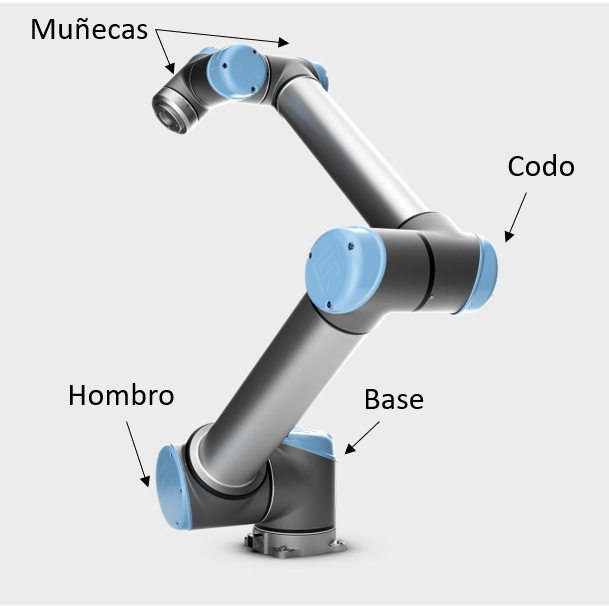
\includegraphics[scale=0.5]{figuras/articulaciones_UR.png}
        %%\caption{Articulaciones del UR}
        \label{fig:articulaciones_UR}
    \end{subfigure}
    \hfill
    \begin{subfigure}[h!]{0.7\textwidth}
        \begin{tabular}{|l|r|}
            \hline
            Carga máxima & 10 kg \\
            \hline
            Alcance máximo & 1300 mm \\
            \hline
            Giro de articulaciones & ± 360º \\
            \hline
            Grados de libertad & 6 \\
            \hline
            Huella & 190 mm \\
            \hline
            Temperatura de trabajo & 0-50 ºC \\
            \hline
            Repetibilidad & ± 5 mm \\
            \hline
            Error de trayectoria \footnote{Medido en el laboratorio} & 0,2 mm \\
            \hline
            Velocidad de giro de base y hombro & 120 º/s \\
            \hline
            Velocidad de giro de codo y muñeca & 180 º/s \\
            \hline
        \end{tabular}
        %%\caption{Valores característicos}
        \label{tab:caracteristicas_UR_tabla}
    \end{subfigure}
    \caption{Características del UR10 \cite{UR_Technical_Specs}}
    \label{tab:caracteristicas_UR}
\end{table}




\subsection{Placa de desarrollo}
La placa de desarrollo utilizada ha sido la ROCK PI 4C+, se trata de una placa de desarrollo desarrollada por la compañia Radxa para brindar potencia de cómputo en un espacio reducido y con conexión a multitud de periféricos. 

Este tipo de placas están basadas en la arquitectura ARM y son ampliamente utilizadas en proyectos donde se necesitan programar cirucitos integrados de forma flexible y rápida. Las placas Rock Pi pueden variar en términos de hardware, pero suelen incluir puertos HDMI, USB, conectividad Ethernet y soporte para tarjetas microSD. Algunos modelos pueden tener capacidades inalámbricas, como Wi-Fi y Bluetooth. 
Estas placas son conocidas por su versatilidad y su capacidad para ejecutar sistemas operativos Linux, haciéndolas idóneas para opciones desarrollo enfocadas en altos rendimientos a bajo costo que sigan la filosofía \acrshort{SBC} \cite{web_rockpi}.

\begin{figure}[h!]
    \centering
    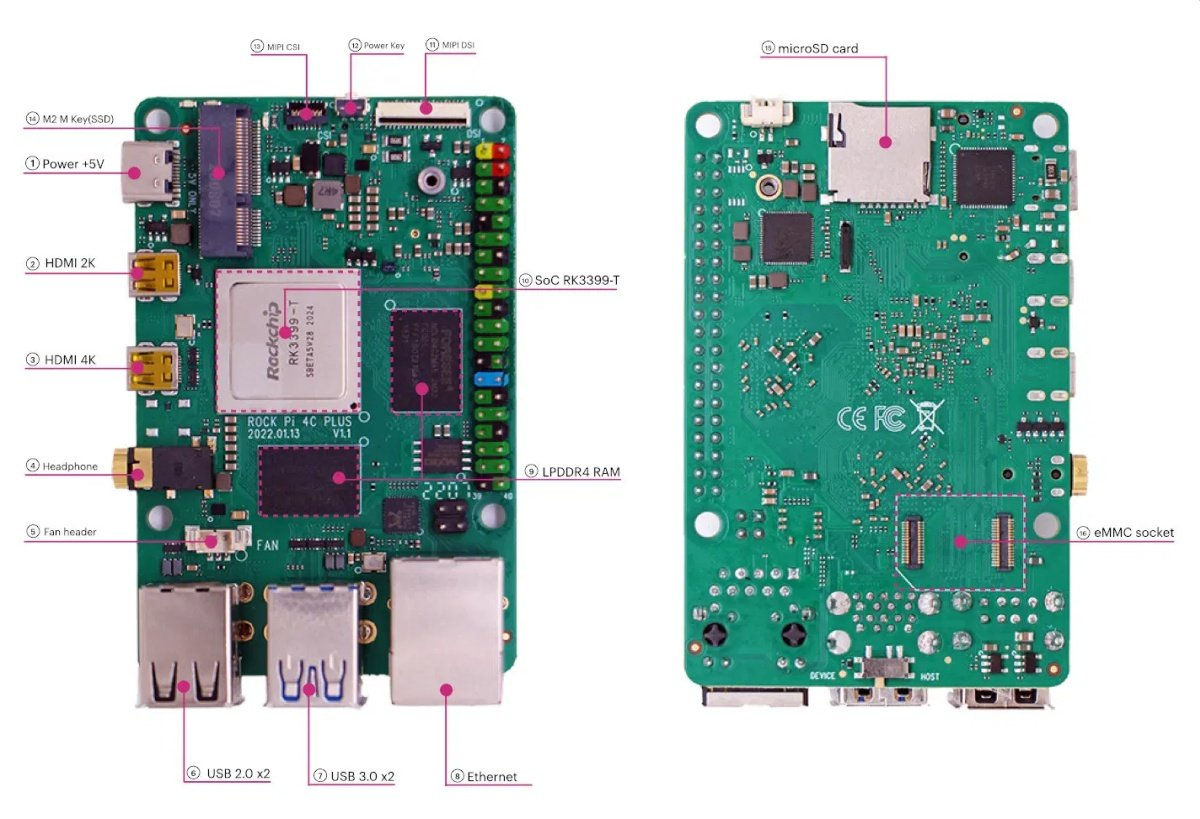
\includegraphics[scale=0.15]{figuras/rock-pi-model-c-plus_06.jpg}
    \caption{Esquema de una placa Rock Pi 4.}
    \label{fig:rockpi_esquema}
\end{figure}

\section{Software}

\begin{figure}[t!]
\centerline{\includesvg[width=\columnwidth]{figuras/Diagramas TFM.svg}}
\caption{Example of using SVG on Overleaf}
\label{fig: example}
\end{figure}